%=======================================================================
%  CSE558 Data Science - Midterm Project Report Template
%  Monsoon 2026, IIIT-Delhi
%
%  How to use this template
%   1. Set your project title in the EDIT THIS block below.
%   2. Replace everything in LIGHT BLUE with your own text and numbers.
%      The numbers in the example are made up for illustration.
%   3. Grey italic lines are instructions. Delete them as you write, or
%      hide them all at once with \showhintsfalse.
%   4. Upload your plots to the project and put their file names in
%      \figfile{...}{...}. Until a file exists, a labelled box is shown.
%
%  Sections 1-5 follow items 1-5 of the report guidelines; Section 6 is
%  the limitations of your analysis. The link to your code (item 6) goes
%  at the top. At most 8 pages.
%  Compile with pdfLaTeX (Overleaf's default setting works), twice.
%=======================================================================
\documentclass[10pt,a4paper,twocolumn]{article}

%========================= EDIT THIS =========================
% Your project title: it sets the heading AND the PDF's title.
\newcommand{\projecttitle}{What Changes a Mind? Length, Timing and Evidence on r/ChangeMyView}
\newif\ifshowhints
\showhintsfalse      % \showhintsfalse hides every grey instruction line
%=============================================================

%-------------------------------------------- fonts (no need to edit)
\usepackage{iftex}
\ifPDFTeX
  \usepackage[T1]{fontenc}
  \usepackage[utf8]{inputenc}
  \IfFileExists{carlito.sty}%
    {\usepackage[sfdefault]{carlito}}%              Calibri look
    {\usepackage[scaled=0.92]{helvet}\renewcommand{\familydefault}{\sfdefault}}%
  \usepackage{courier}
\else
  \usepackage[no-math]{fontspec}
  \setmainfont{Carlito}[Extension=.ttf, UprightFont=*-Regular, BoldFont=*-Bold,
    ItalicFont=*-Italic, BoldItalicFont=*-BoldItalic]
\fi

%----------------------------------------------------------- packages
\usepackage[margin=18mm,bottom=20mm,columnsep=7mm]{geometry}
\usepackage{amsmath}
\usepackage{xcolor}
\usepackage{graphicx}
\usepackage{tabularx}
\usepackage{array}
\usepackage{booktabs}
\usepackage{enumitem}
\usepackage{titlesec}
\usepackage{needspace}
\usepackage{balance}
\usepackage[font=small,labelfont=bf]{caption}
\usepackage[hidelinks]{hyperref}
\hypersetup{pdftitle={\projecttitle},
            pdfsubject={CSE558 Data Science, Monsoon 2026: Midterm Project Report}}

%------------------------------------------------------------- layout
\definecolor{eg}{HTML}{7396C4}         % worked example (light blue)
\definecolor{hintgrey}{gray}{0.58}     % instructions (light grey)

\titleformat{\section}{\normalfont\large\bfseries}{\thesection.}{0.5em}{}
\titlespacing*{\section}{0pt}{12pt}{3pt}
\titleformat{\subsection}{\normalfont\normalsize\bfseries}{\thesubsection}{0.5em}{}
\titlespacing*{\subsection}{0pt}{10pt}{2pt}
\newcommand{\sectionbreak}{\needspace{10\baselineskip}}
\newcommand{\subsectionbreak}{\needspace{10\baselineskip}}

\setlength{\parindent}{0pt}
\setlength{\parskip}{4pt}
\setlist{leftmargin=1.2em, itemsep=2pt, topsep=2pt, parsep=0pt}
\renewcommand{\arraystretch}{1.25}
\setlength{\tabcolsep}{4pt}
\newcolumntype{L}[1]{>{\raggedright\arraybackslash}p{#1}}
\newcolumntype{Y}{>{\raggedright\arraybackslash}X}
\newcolumntype{K}[1]{>{\raggedright\arraybackslash\bfseries\boldmath}p{#1}}  % bold labels

%--------------------------------------------------------- shorthands
% Instruction line. Delete these as you fill the template in.
\newcommand{\hint}[1]{\ifshowhints{\footnotesize\itshape\color{hintgrey}#1\par}\fi}
% Worked example: inline or in a table cell. REPLACE the contents.
\newcommand{\eg}[1]{\textcolor{eg}{#1}}
% Worked example running over a whole paragraph.
\newcommand{\egblock}[1]{{\color{eg}#1\par}}
% Bold label followed by an example.
\newcommand{\field}[2]{\textbf{#1}~\eg{#2}\par}
% Part a)-c) of a test, and a small bold heading.
\newcommand{\tpart}[2]{\par\needspace{12\baselineskip}\smallskip\textbf{#1)~#2}\par}
\newcommand{\minihead}[1]{\par\needspace{8\baselineskip}\smallskip\textbf{#1}\par}
% Column and file names.
\newcommand{\code}[1]{\texttt{#1}}
% \figfile{file}{height}: your plot, or a labelled box until the file exists.
\newcommand{\figfile}[2]{%
  \IfFileExists{#1}%
    {\includegraphics[width=\linewidth,height=#2,keepaspectratio]{#1}}%
    {\fbox{\parbox[c][#2][c]{\dimexpr\linewidth-2\fboxsep-2\fboxrule\relax}%
      {\centering\small\itshape\color{hintgrey}Your plot: \detokenize{#1}}}}}

%=======================================================================
\renewcommand{\eg}[1]{#1}
\renewcommand{\egblock}[1]{{#1\par}}
\begin{document}

\twocolumn[%
{\small\bfseries CSE558 Data Science\ \ \textbullet\ \ Midterm Project Report\ \ \textbullet\ \ Monsoon 2026\par}
\vspace{4pt}
{\LARGE\bfseries\raggedright\projecttitle\par}
\vspace{6pt}
\rule{\linewidth}{1pt}

{\small
\begin{tabularx}{\linewidth}{@{}K{2.4cm} Y@{}}
\toprule
Group name & DataMindz \\
Dataset & r/ChangeMyView archive (raw coverage: 2013--2025; analysis window: Apr 2017--Nov 2022) \\
Code & \url{https://github.com/pranaybansal19/Data-Science-Project} (notebook \code{CMV\_Analysis.ipynb} and README) \\
\bottomrule
\end{tabularx}}
\vspace{2pt}
{\small
\begin{tabularx}{\linewidth}{@{}L{0.5cm} L{3.4cm} L{2.3cm} L{4.8cm} Y@{}}
\toprule
\textbf{\#} & \textbf{Name} & \textbf{Roll no.} & \textbf{Institute email} & \textbf{Contribution} \\
\midrule
1 & Karan Singh & 2023273 & karan23273@iiitd.ac.in & Dataset review and size validation \\
2 & Dhruv Jain & 2023198 & dhruv23198@iiitd.ac.in & Data preparation and before/after analysis \\
3 & Akshat Singh & 2023064 & akshat23064@iiitd.ac.in & Exploratory analysis and problem statements \\
4 & Pranay Bansal & 2023343 & pranay23343@iiitd.ac.in & Hypothesis Tests 1 and 2 \\
5 & Somesh Singh & PhD & somesh@iiitd.ac.in & Tests 3 and 4, limitations, code and documentation \\
\bottomrule
\end{tabularx}}
\vspace{12pt}
]

%-----------------------------------------------------------------------
\section{Dataset}

\field{Source and coverage:}{the raw \href{https://www.reddit.com/r/changemyview/}{r/ChangeMyView (CMV)} archive was obtained with the \href{https://arctic-shift.photon-reddit.com/download-tool}{Arctic Shift Reddit Download Tool}. It covers January 2013 through December 2025; this is the archive coverage, not the analysis period. After quality and consistency filters, all descriptive results and hypothesis tests use posts from 1 April 2017 through 30 November 2022. In CMV, an original poster (OP) may award a delta ($\Delta$) to a reply that changes their view, and DeltaBot records the award in a confirmation comment.}

\field{Raw-data challenges:}{the archive has no ready-made outcome column: delta awards appear only inside DeltaBot comments. Many post and reply bodies are deleted or removed, schemas vary across years, 2{,}508 comment IDs are duplicated, and IDs change representation in 2023. Across the complete files we observed 132 post fields and 81 comment fields.}

The notebook streams both compressed archives once and retains only the fields required for filtering, reconstruction, exploratory analysis and hypothesis tests. This avoids loading 18.6 million complete comment objects into memory.

{\small
\begin{tabularx}{\linewidth}{@{}L{3.0cm} Y Y@{}}
\toprule
 & \textbf{Raw files} & \textbf{After encoding} \\
\midrule
Instances (rows) & 345{,}098 posts, 18{,}644{,}355 comments & 479{,}276 replies \\
Attributes (columns) & 132 / 81 & 11 \\
\bottomrule
\end{tabularx}}

\field{Size check:}{$479{,}276\times11=5{,}272{,}036\ge3{,}000{,}000$. Each row is one eligible top-level reply. The 11 encoded attributes contain reply length and its log transform, response delay, five delay indicators, a link indicator, post length and the binary outcome.}

\minihead{Selected analytical features}
{\footnotesize
\begin{tabularx}{\linewidth}{@{}L{2.0cm} L{1.5cm} Y@{}}
\toprule
\textbf{Feature} & \textbf{Type} & \textbf{Real-world meaning} \\
\midrule
\code{won} & binary, reply & direct OP award, or a later OP award to the opening author's comment in the same branch \\
\code{words} & discrete, reply & whitespace-separated token count in the reply \\
\code{log\_words} & continuous, reply & $\log(1+\code{words})$, used for length inference \\
\code{delay\_h} & continuous, reply & hours from the post to the reply \\
delay indicators & five binary columns & $<$1, 1--3, 3--6, 6--24 and $>$24 hours \\
\code{has\_link} & binary, reply & text contains \code{http://}, \code{https://} or \code{www.} \\
\code{post\_words} & discrete, reply & whitespace-separated token count in the original post \\
\code{op\_awarded} & binary, thread & OP gave at least one delta; used for Test 4, not part of the 11-column reply table \\
\bottomrule
\end{tabularx}}

%-----------------------------------------------------------------------
\section{Data preparation}

{\footnotesize
\begin{tabularx}{\linewidth}{@{}L{1.85cm} L{2.35cm} Y@{}}
\toprule
\textbf{Issue found} & \textbf{What we did} & \textbf{Why, and not the alternative} \\
\midrule
no outcome column
 & rebuilt it: DeltaBot ``Confirmed'' $\rightarrow$ the message it confirms must be by the OP and reply to a comment $\rightarrow$ that comment won
 & a $\Delta$ character can occur in quoted or instructional text; requiring an OP-authored award and bot confirmation reduces false labels \\
deltas often land on a later comment in a branch
 & the top-level reply wins if the OP awarded it, or a later comment by the same author in its branch
 & 26{,}573 awards followed a back-and-forth; direct-award matching alone would mislabel those opening replies \\
inconsistent award capture outside the analysis period
 & kept posts from 1 Apr 2017 to 30 Nov 2022
 & this provides a stable observation window and avoids the sharp archive discontinuity visible after 2022 in Figure~\ref{fig:window} \\
mod posts, meta threads
 & kept titles starting with ``CMV''
 & CMV's rules require it, so anything else is not a view \\
NSFW posts
 & dropped (1{,}326 posts)
 & their restricted visibility creates a different exposure process \\
post removed, or OP account deleted
 & thread dropped, not imputed
 & the text or OP identity required for measurement is unavailable; imputing argument text or authorship would be invalid \\
OP never awarded a delta
 & dropped for Tests 1--3, kept for Test 4
 & Tests 1--3 require at least one observed OP award; Test 4 explicitly compares award and non-award threads \\
deleted replies, OP's own, bots and mod notices
 & dropped
 & no text to measure, or not an argument \\
replies under 10 words
 & dropped (20{,}451)
 & an eligibility rule for substantive top-level arguments; it removes 4.1\% of otherwise eligible replies, so results remain conditional on this threshold \\
2{,}508 duplicate comment IDs
 & kept the first copy
 & the same comment counted twice \\
skewed lengths, 5--6\% beyond the IQR fence
 & kept, analysed on $\log(1+x)$
 & long replies are valid observations. The transform reduces skewness from 3.3 to 0.02 and lets differences be interpreted as ratios \\
delay is very skewed
 & binned ($<$1\,h, 1--3, 3--6, 6--24, $>$24\,h), one-hot
 & we compare rates by delay, never average it \\
\bottomrule
\end{tabularx}}

\field{Why this window:}{we retain posts from 1 April 2017 through 30 November 2022. Earlier records have less reliable bot-based award capture, while the series changes sharply after 2022. Within the selected period the quarterly share of intact threads with an OP award is comparatively stable (Figure~\ref{fig:window}), giving the four tests a more consistent measurement regime.}

%-----------------------------------------------------------------------
\section{What changed after preparation}

{\footnotesize
\begin{tabularx}{\linewidth}{@{}L{2.4cm} L{2.2cm} Y@{}}
\toprule
\textbf{Measure} & \textbf{Before} & \textbf{After} \\
\midrule
Posts & 345{,}098 & 44{,}160 intact CMV threads; 25{,}447 where the OP gave a delta \\
Comments $\rightarrow$ replies & 18{,}644{,}355 & 479{,}276 top-level replies \\
Time span & raw archive: Jan 2013--Dec 2025 & analyzed posts: 1 Apr 2017--30 Nov 2022 \\
Outcome & none & \code{won}: 42{,}197 winners (8.8\%) \\
Missing text & 66\% of posts removed & 0 \\
Duplicate IDs & 2{,}508 & 0 \\
\bottomrule
\end{tabularx}}

The largest reduction occurs at thread level because valid post text and OP identity are required. Within retained threads, the pipeline removes 83{,}114 deleted replies, 29{,}204 bot or moderator notices, 166 OP-authored top-level comments and 20{,}451 replies below 10 words. Eight qualifying award threads have no reply remaining after these filters, so 479{,}276 analyzed replies represent 25{,}439 of the 25{,}447 qualifying threads. The final \code{won} field contains 42{,}197 positive outcomes.

%-----------------------------------------------------------------------
\section{Basic questions and problem statement}

\begin{figure}[!ht]
\centering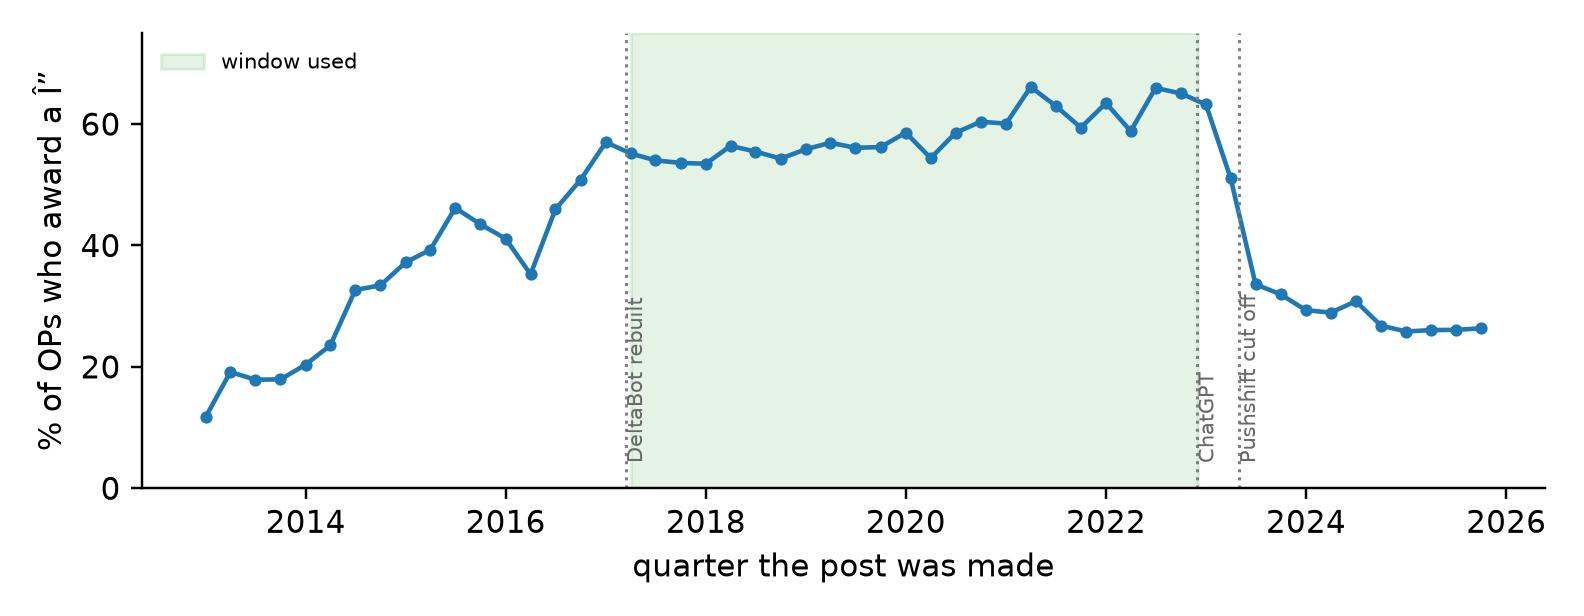
\includegraphics[width=\linewidth]{figures/op_award_share.png}
\caption{Quarterly share of intact CMV threads in which the OP awards a delta. The shaded region is the analysis window; dotted lines mark its boundaries and the later archive discontinuity.}\label{fig:window}
\end{figure}

\begin{figure}[!ht]
\centering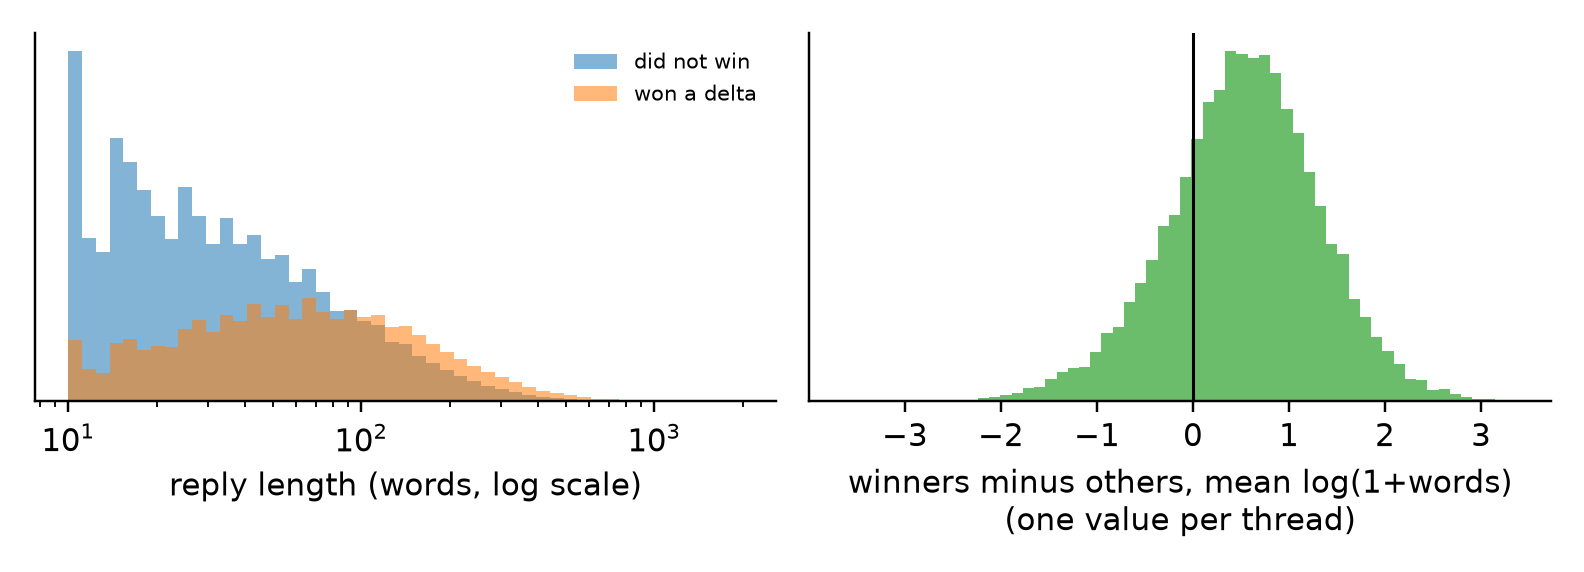
\includegraphics[width=\linewidth]{figures/length.png}
\caption{Reply length and outcome. Left: distributions for winning and non-winning replies on a log scale. Right: within-thread difference between winners and other replies; positive values mean winners are longer.}\label{fig:len}
\end{figure}

\begin{figure}[!ht]
\centering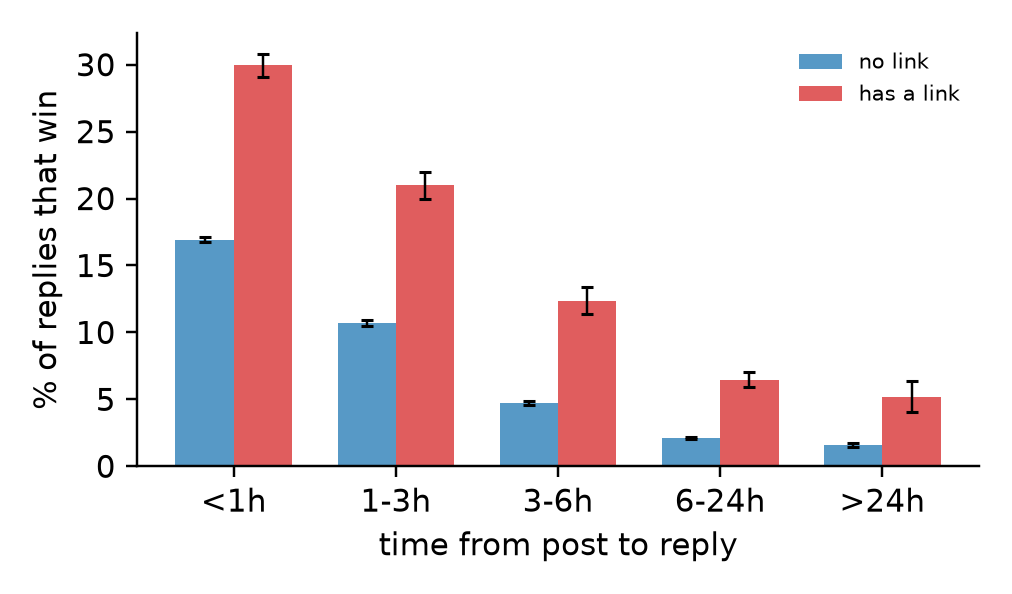
\includegraphics[width=0.82\linewidth]{figures/delay_link.png}
\caption{Win rate by response-delay bin and link status. Error bars show 95\% confidence intervals. Earlier replies and replies containing a link have higher observed win rates.}\label{fig:delay}
\end{figure}

\minihead{Basic questions}
\begin{enumerate}[label=\arabic*.]
  \item How long are replies, and how soon do they arrive? Median 84 words, 3.8\,h after the post; 6.2\% contain a link.
  \item How many OPs award a delta? 57.6\% of the 44{,}160 intact threads.
  \item How many retained replies win? 42{,}197 of 479{,}276, or 8.8\%. The observed rate declines as response delay increases.
\end{enumerate}

\minihead{Our problem statements}
\noindent\fbox{\begin{minipage}{\dimexpr\linewidth-2\fboxsep-2\fboxrule\relax}
\textbf{P1 (primary).} Within the same thread, are the replies that win a delta longer than the ones that don't?

\smallskip
\textbf{P2.} Do replies posted within 3 hours of the post win more often than later ones?

\smallskip
\textbf{P3.} Do replies that link to a source win more often?

\smallskip
\textbf{P4.} Do OPs who explain their view at greater length award a delta more often, or less?
\end{minipage}}

\field{Analytical contribution:}{the pipeline reconstructs an explicit persuasion outcome from bot confirmations and reply trees. P1 controls for thread context through paired comparisons, P2 and P3 test timing and linked evidence, and P4 shifts the unit of analysis from replies to OP-authored threads.}

%-----------------------------------------------------------------------
\section{Statistical inferences}

\field{Rows tested:}{Tests 1--3 use 479{,}276 retained replies from 25{,}439 represented threads, drawn from the 25{,}447 qualifying threads where the OP gave a delta. Test 4 uses all 44{,}160 intact threads. Every statistic is computed from the lecture formula and checked against \code{scipy}.}

\field{Practical-effect thresholds:}{for length comparisons we use a ratio of 1.20; for win-rate comparisons we use 2 percentage points, approximately 20\% of the 8.8\% base rate. Statistical significance is reported separately from whether an estimate crosses these practical thresholds.}

%------------------------------------------------------------ Test 1
\subsection*{Test 1 (P1): within a thread, are winning replies longer?}

\tpart{a}{Hypotheses and test design}
{\small
\begin{tabularx}{\linewidth}{@{}K{3.4cm} Y@{}}
\toprule
$H_0$ & $\mu_d\le0$ \\
$H_1$ & $\mu_d>0$ \\
Significance level & $\alpha=0.05$ \\
Side & one-sided (right) \\
Test & paired t-test \\
Smallest difference that matters & winners 20\% longer: $\mu_d\ge\ln1.20=0.182$ \\
\bottomrule
\end{tabularx}}

For every eligible thread, $d$ is the mean $\log(1+\text{words})$ among winners minus the corresponding mean among other replies. The paired design compares replies judged in the same discussion and removes between-thread differences in topic and OP.

\tpart{b}{Other tests we considered}
The paired t-test directly matches P1 and the dependence structure. The 23{,}055 thread-level differences are nearly symmetric (skewness $-0.20$), and the large sample makes inference on their mean stable.
{\footnotesize
\begin{tabularx}{\linewidth}{@{}L{2.4cm} Y@{}}
\toprule
\textbf{Also considered} & \textbf{Why we did not use it} \\
\midrule
Welch t-test (unpaired) & ignores the thread, so busy threads full of short replies dominate. Run anyway: ratio 1.77, $t=126.8$, same decision \\
Pooled t-test & also unpaired, and an F-test rejects equal variances ($F=0.83$, $p<10^{-100}$) \\
Two-sample z-test & needs the population $\sigma$, which we do not know \\
$\chi^2$ on length bins & throws away the size of the gap and depends on where we cut \\
\bottomrule
\end{tabularx}}

\tpart{c}{Result}
{\small
\begin{tabularx}{\linewidth}{@{}K{3.4cm} Y@{}}
\toprule
Estimate & $\bar d=0.519$: winners are 1.68$\times$ as long \\
95\% confidence interval & 1.66$\times$ to 1.70$\times$ \\
Test statistic (d.f.) & $t=98.4$ (23{,}054) \\
p-value & $<10^{-300}$ \\
Decision & reject $H_0$ \\
\bottomrule
\end{tabularx}}

Within the same thread, winning replies are estimated to be 1.68 times as long as other replies. The entire interval exceeds the 1.20 threshold. This is a strong association, but it does not show that adding words alone causes persuasion.

%------------------------------------------------------------ Test 2
\subsection*{Test 2 (P2): do early replies win more often?}

\tpart{a}{Hypotheses and test design}
{\small
\begin{tabularx}{\linewidth}{@{}K{3.4cm} Y@{}}
\toprule
$H_0$ & $p_{\text{early}}-p_{\text{late}}\le0$ \\
$H_1$ & $p_{\text{early}}-p_{\text{late}}>0$ \\
Significance level & $\alpha=0.05$ \\
Side & one-sided (right) \\
Test & two-proportion z-test \\
Smallest difference that matters & 2 percentage points \\
\bottomrule
\end{tabularx}}

$p_{\text{early}}$ and $p_{\text{late}}$ are the winning proportions for replies posted within 3 hours and after 3 hours. The cutoff is close to the median delay and produces two large groups: 219{,}836 early and 259{,}440 late replies.

\tpart{b}{Other tests we considered}
Both groups contain far more than 15 successes and failures, satisfying the large-sample condition for a two-proportion z-test.
{\footnotesize
\begin{tabularx}{\linewidth}{@{}L{2.4cm} Y@{}}
\toprule
\textbf{Also considered} & \textbf{Why we did not use it} \\
\midrule
$\chi^2$ independence, 5 delay bins & tells us the rate depends on delay, but not in which direction or by how much. Run anyway: $\chi^2=26{,}641$ (4), and the rate falls in every bin (Figure~\ref{fig:delay}) \\
$2\times2$ $\chi^2$ & the same test: $\chi^2=z^2$ \\
Welch t on delay & asks the reverse question (does winning predict delay?) and averages a very skewed variable \\
Paired t across threads & also valid, and it handles replies sharing a thread. Run as a check: +13.3 points, $t=80.1$ (22{,}781), same decision \\
\bottomrule
\end{tabularx}}

\tpart{c}{Result}
{\small
\begin{tabularx}{\linewidth}{@{}K{3.4cm} Y@{}}
\toprule
Estimate & $+12.6$ points (15.6\% early, 3.0\% late) \\
95\% confidence interval & $+12.4$ to $+12.8$ points \\
Test statistic & $z=153.5$ \\
p-value & $<10^{-300}$ \\
Decision & reject $H_0$ \\
\bottomrule
\end{tabularx}}

Early replies have a 12.6-point higher observed win rate and win about five times as often as later replies. The confidence interval lies well above the 2-point threshold. Timing remains observational and may also reflect visibility or reply quality.

%------------------------------------------------------------ Test 3
\subsection*{Test 3 (P3): do replies with a link win more often?}

\tpart{a}{Hypotheses and test design}
{\small
\begin{tabularx}{\linewidth}{@{}K{3.4cm} Y@{}}
\toprule
$H_0$ & $p_{\text{link}}-p_{\text{none}}\le0$ \\
$H_1$ & $p_{\text{link}}-p_{\text{none}}>0$ \\
Significance level & $\alpha=0.05$ \\
Side & one-sided (right) \\
Test & two-proportion z-test \\
Smallest difference that matters & 2 percentage points \\
\bottomrule
\end{tabularx}}

The alternative tests whether replies containing at least one URL have a higher win rate. The link indicator measures the presence of a link, not the credibility or relevance of its destination.

\tpart{b}{Other tests we considered}
The linked and unlinked groups contain 29{,}653 and 449{,}623 replies respectively, with enough successes and failures for the normal approximation.
{\footnotesize
\begin{tabularx}{\linewidth}{@{}L{2.4cm} Y@{}}
\toprule
\textbf{Also considered} & \textbf{Why we did not use it} \\
\midrule
$2\times2$ $\chi^2$ & equivalent ($\chi^2=z^2=3{,}645$), but two-sided only \\
Same z-test within length quartiles & not a replacement but a check, since linked replies are longer: the gap is 5.4 to 8.6 points in every quartile \\
Paired t-test & most threads have no linked reply to pair \\
\bottomrule
\end{tabularx}}

\tpart{c}{Result}
{\small
\begin{tabularx}{\linewidth}{@{}K{3.4cm} Y@{}}
\toprule
Estimate & $+10.3$ points (18.4\% with a link, 8.2\% without) \\
95\% confidence interval & $+9.8$ to $+10.7$ points \\
Test statistic & $z=60.4$ \\
p-value & $<10^{-300}$ \\
Decision & reject $H_0$ \\
\bottomrule
\end{tabularx}}

Replies with a link have a 10.3-point higher observed win rate. The gap remains positive within every reply-length quartile and exceeds the practical threshold, although residual differences in topic, author effort and evidence quality may remain.

%------------------------------------------------------------ Test 4
\subsection*{Test 4 (P4): do OPs with longer posts award more?}

\tpart{a}{Hypotheses and test design}
{\small
\begin{tabularx}{\linewidth}{@{}K{3.4cm} Y@{}}
\toprule
$H_0$ & $\mu_{\text{award}}-\mu_{\text{none}}=0$ \\
$H_1$ & $\mu_{\text{award}}-\mu_{\text{none}}\ne0$ \\
Significance level & $\alpha=0.05$ \\
Side & two-sided \\
Test & Welch t-test \\
Smallest difference that matters & posts 20\% longer (or shorter) \\
\bottomrule
\end{tabularx}}

$\mu_{\text{award}}$ and $\mu_{\text{none}}$ are mean $\log(1+\text{post words})$ for threads in which the OP did and did not award a delta. A two-sided alternative allows either group to write longer posts.

\begin{figure}[!ht]
\centering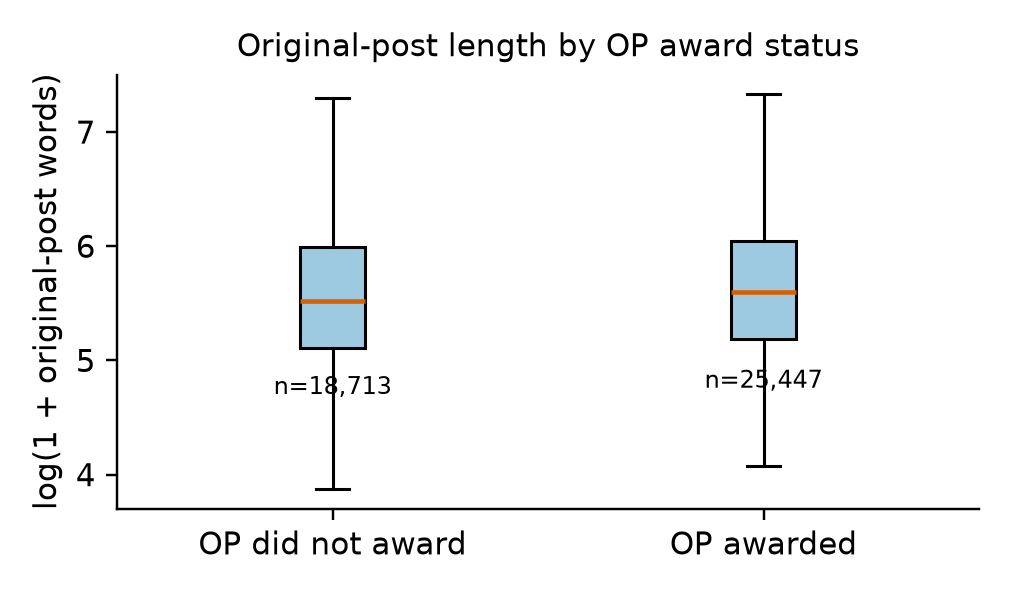
\includegraphics[width=0.92\linewidth]{figures/post_length_award.png}
\caption{Test 4 comparison of original-post length by OP award status. Length is shown on the $\log(1+x)$ scale used by Welch's t-test; outlier markers are hidden for readability, while all observations remain in the test.}\label{fig:postaward}
\end{figure}

\tpart{b}{Other tests we considered}
The two groups are independent and their population variances are unknown. Welch's t-test estimates the mean difference without requiring equal variances.
{\footnotesize
\begin{tabularx}{\linewidth}{@{}L{2.4cm} Y@{}}
\toprule
\textbf{Also considered} & \textbf{Why we did not use it} \\
\midrule
Pooled t-test & assumes equal variances, which the F-test rejects ($F=0.955$, $p=0.0007$). Run anyway: $t=11.03$, same decision \\
Two-sample z-test & needs the population $\sigma$ \\
Two-proportion z on award rate, long vs short posts & cuts length at an arbitrary point. Run anyway: 60.1\% vs 55.2\% \\
Paired t-test & each thread has one OP; nothing to pair \\
\bottomrule
\end{tabularx}}

\tpart{c}{Result}
{\small
\begin{tabularx}{\linewidth}{@{}K{3.4cm} Y@{}}
\toprule
Estimate & posts 1.07$\times$ as long (medians 270 vs 248 words) \\
95\% confidence interval & 1.06$\times$ to 1.08$\times$ \\
Test statistic (d.f.) & $t=10.99$ (39{,}789) \\
p-value & $4.5\times10^{-28}$ \\
Decision & reject $H_0$ \\
\bottomrule
\end{tabularx}}

Awarding OPs write slightly longer posts on average, but the estimated ratio of 1.07 and its confidence interval remain well below the 1.20 practical threshold. The large sample detects a statistically clear difference that is small in magnitude.

%-----------------------------------------------------------------------
\balance
\section{Limitations}
{\footnotesize
\begin{itemize}[leftmargin=1.1em,itemsep=1pt,topsep=1pt]
\item \textbf{Association, not causation.} Reply length, timing and links may reflect effort, topic, visibility or argument quality; the tests do not isolate causal effects.
\item \textbf{Dependence.} Replies share an OP and discussion context, so reply-level z-tests may understate uncertainty. Thread-level checks support the same directions.
\item \textbf{Measurement and selection.} Deltas are public acknowledgements reconstructed from bot comments. Unreported changes of mind are invisible, and Tests 1--3 condition on intact threads with at least one OP award.
\item \textbf{Short-reply threshold.} The 10-word rule removes non-substantive messages but is still a modeling choice. A full sensitivity analysis at 0, 5 and 10 words would show whether conclusions depend on it.
\item \textbf{Time period.} Results describe April 2017 through November 2022 and may not generalize to later CMV activity.
\end{itemize}}

\end{document}
